\chapter{How does X Influence Novelty, Complexity, and Adaptation?}
\label{ch:influencing-cna}

\noindent
% Authors: Matthew Andres Moreno, Santiago Rodriguez Papa, and Charles Ofria \\
This chapter is a proposal.

\section{Introduction}

SignalGP is a biologically-inspired approach that allows digital organisms to dynamically respond to environmental signals.
Each event (i.e., a signal from the environment or other agent) is associated with a tag to identify it; modules in the digital organism will be triggered to execute when an event with a matching tag occurs (Figure \ref{fig:signalgp-schematic;ch:influencing-cma}) \citep{lalejini2018evolving}.

Previous work has shown that SignalGP allows evolved programs to engage in a broad range of environmental interactions and can better incorporate context into their behaviors.
Lalejini et. al. found that tag-based genetic regulation dramatically improved the solution success rate on sensor-intensive and context-dependent problems \citep{lalejini2018evolving, lalejini2021tag}.
Despite these positive results, this methodology has not yet been directly examined in an artificial life context, especially for its capacity to produce biologically realistic interactions.
Our goal is to enrich the toolbox of artificial life researchers to conduct evolution experiments while also expanding the applications to genetic programming.

\begin{figure}[h]

\centering
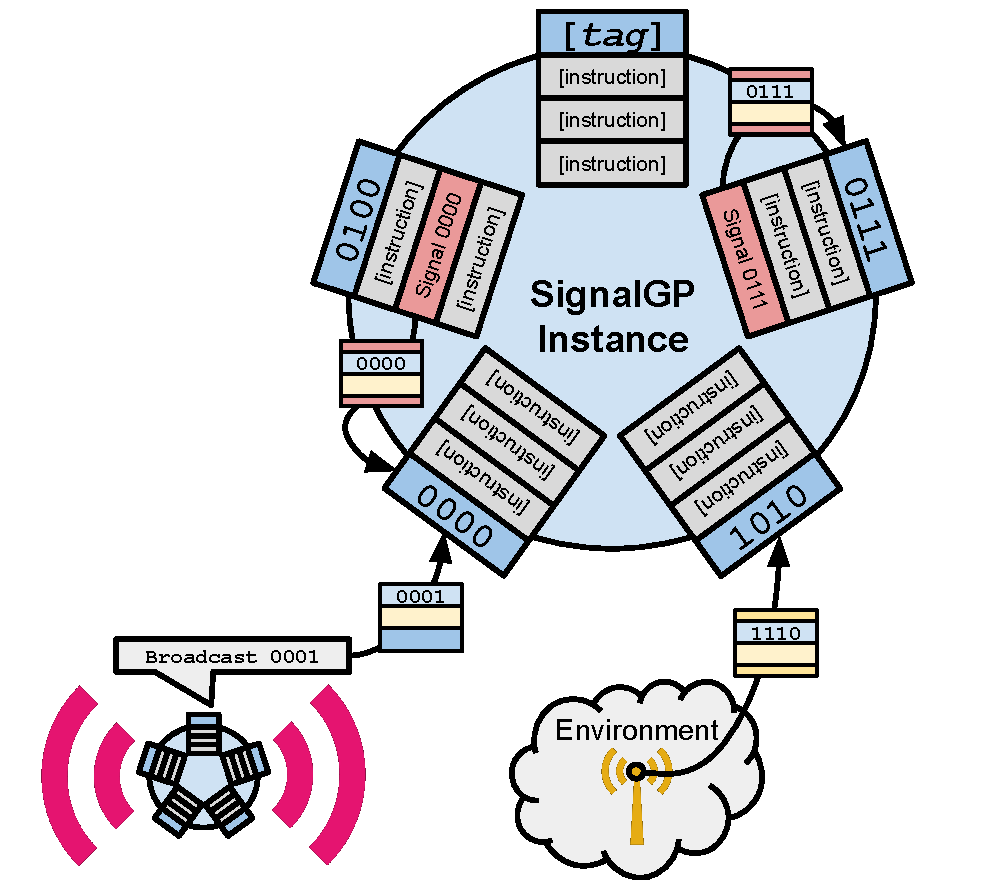
\includegraphics[width=0.5\textwidth]{img/signalgp-schematic}

\caption{SignalGP schematic depicting interactions between an agent and its environment}
\label{fig:signalgp-schematic;ch:influencing-cna}

\end{figure}


DISHTINY is a digital framework designed to study open-ended transitions to multicellularity \citep{moreno2019toward}.
In preliminary studies, we have used SignalGP in DISHTINY to enable dynamic interactions among cells and between cells and their environment, resulting in complex and diverse multi-cellular organisms.
Existing work with DISHTINY has focused on studying the evolution of multicellular traits, but not on characterizing the genetic programming representation that underpins it.

I propose to use DISHTINY to test whether an event-driven encoding can facilitate evolution of greater
\begin{itemize}
  \item fitness,
  \item interface complexity, and
  \item genetic robustness
\end{itemize}
in an artificial life context.

\section{Proposed Work}

Our experimental treatment will provide all inputs via both
\begin{itemize}
  \item a sensor instruction, and
  \item a corresponding event signal.
\end{itemize}
Agents will able to communicate with neighbors by both
\begin{itemize}
  \item dispatching arbitrarily-tagged message events to neighbors, and
  \item writing to placebo output registers visible to neighbors via sensor instructions.
\end{itemize}

We will conduct two control treatments where we modify signal function on multicellular organisms to isolate the impact of these event-driven cues.

In a first control treatment, we will disable event signals from both the environment and from messages dispatched between agents.
This control treatment will retain messaging instructions, but render them ineffectual.
All information exchange between agents and the environment will be restricted to register-based input and output.
However, agents will still be allowed to generate and process internal events (i.e., fork and jump instructions).

In the second control treatment, we will retain event signals but strip their context.
Instead of receiving their own environmental cues, cells will receive environmental cues generated for another arbitrary cell located on the same processor.
Messaging instructions will dispatch message events back to the sender (``self-send'') instead of a neighbor.
This treatment will allow the effect of event-driven signals in conveying meaningful information to be isolated from any contingent effects of simply providing general opportunities to trigger execution of genome code.

We will assess the impact of event-driven cues between treatments in terms of:
\begin{enumerate}
  \item the number of distinct cues from environmental factors and other agents incorporated into adaptive behaviors,
  \label{itm:interface-complexity;ch:influencing-cna}
  \item overall fitness of evolved behavioral strategies, and
  \label{itm:fitness;ch:influencing-cna}
  \item robustness of evolved behaviors under mutation.
  \label{itm:robustness;ch:influencing-cna}
\end{enumerate}

The interface complexity measure described in Sections \ref{sec:estimating-state-interface-complexity;ch:measuring-cna} and \ref{sec:messaging-state-interface-complexity;ch:measuring-cna} will be used for Item \ref{itm:interface-complexity;ch:influencing-cna}.

Evaluating question \label{itm:fitness;ch:influencing-cna} will require a proxy for fitness, because fitness within DISHTINY is implicit and so can not be measured directly.
Competition experiments will serve as a fitness proxy.
However, competitive superiority is not necessarily well-ordered among DISHTINY strains.
In exploratory work, we have anecdotally observed occasional rock-paper-scissors fitness cycles (where $\mathrm{fit}(a) > \mathrm{fit}(b)$ and $\mathrm{fit}(b) > \mathrm{fit}(c)$ yet $\mathrm{fit}(c) > \mathrm{fit}(a)$).
For this reason, we will perform a tournament where each strain from the experimental treatment can compete against several control strains and vice versa.
To evaluate whether one treatment enjoys an overall fitness advantage, we will quantify each strain's fraction of competitions won then perform a between Mann-Whitney $U$ test the two treatments.
This should be more conservative than simply using a binomial test on net competitions won for each treatment.

Finally, I propose a three-pronged approach to evaluating Item \label{itm:robustness;ch:influencing-cna}.
To characterize evolved solutions' one-step mutational neighborhood, we can can evaluate the fraction of mutations that are significantly deleterious (via competition experiments) and the mean magnitude of fitness degradation under mutation (from those same competition experiments).
To characterize the broader mutational neighborhood, we can run competition experiments between mutation-enabled and mutation-disabled variants of strains.

Establishing how SignalGP affects these metrics is critical to understanding how to effectively employ it, and will ultimately advance experimentally-driven studies of evolution in action.

\section{Challenges}

\begin{figure}
\begin{center}

\begin{subfigure}[b]{\textwidth}
\centering
\includegraphics[width=0.6\textwidth]{submodules/dishtiny/binder/bucket=prq49/a=all_stints_all_series_profiles+endeavor=16/teeplots/bucket=prq49+endeavor=16+hue=series+transform=filter-Stint-mod10+viz=lineplot+x=stint+y=cardinal-interface-complexity+ext=}%
\caption{
Lines track individual replicates
}
\label{fig:cardinal-interface-complexity-vs-stint-lineplot}
\end{subfigure}

\begin{subfigure}[b]{\columnwidth}
\centering
\includegraphics[width=0.6\textwidth]{submodules/dishtiny/binder/bucket=prq49/a=all_stints_all_series_profiles+endeavor=16/teeplots/bucket=prq49+endeavor=16+transform=filter-Stint-mod10+viz=swarmplot-boxplot+x=stint+y=cardinal-interface-complexity+ext=}
\caption{
Boxplots with individual replicates overlaid as dots
}
\label{fig:cardinal-interface-complexity-vs-stint-boxplot}
\end{subfigure}

\begin{subfigure}[b]{\columnwidth}
\centering
\includegraphics[width=0.6\textwidth]{submodules/dishtiny/binder/bucket=prq49/a=all_stints_all_series_profiles+endeavor=16/teeplots/bucket=prq49+endeavor=16+transform=filter-Stint-mod10+viz=barplot+x=stint+y=cardinal-interface-complexity+ext=}
\caption{
Error bars represent bootstrapped 95\% confidence intervals
}
\label{fig:cardinal-interface-complexity-vs-stint-barplot}
\end{subfigure}

\caption{
Cardinal interface complexity for 40 replicates over 100 three hour evolutionary stints.
Cardinal interface complexity sums inter-messaging complexity, intra-messaging complexity, and state interface complexity.
}
\label{fig:cardinal-interface-complexity-vs-stint}

\end{center}
\end{figure}

\begin{figure}
\begin{center}

\begin{subfigure}[b]{\textwidth}
\centering
\includegraphics[width=0.6\textwidth]{submodules/dishtiny/binder/bucket=prq49/a=all_stints_all_series_profiles+endeavor=16/teeplots/bucket=prq49+endeavor=16+hue=series+transform=filter-Stint-mod10+viz=lineplot+x=stint+y=num-less-fit-under-inter-self-send-filter-mod-20+ext=}%make ma
\caption{
Lines track individual replicates
}
\label{fig:inter-messaging-complexity-vs-stint-lineplot}
\end{subfigure}

\begin{subfigure}[b]{\columnwidth}
\centering
\includegraphics[width=0.6\textwidth]{submodules/dishtiny/binder/bucket=prq49/a=all_stints_all_series_profiles+endeavor=16/teeplots/bucket=prq49+endeavor=16+transform=filter-Stint-mod10+viz=swarmplot-boxplot+x=stint+y=num-less-fit-under-inter-self-send-filter-mod-20+ext=}
\caption{
Boxplots with individual replicates overlaid as dots
}
\label{fig:inter-messaging-complexity-vs-stint-boxplot}
\end{subfigure}

\caption{
Intercellular messaging complexity for 40 replicates over 100 three hour evolutionary stints.
Intercellular messaging complexity counts the number of distinct intercellular message tags that cause a fitness penalty when re-routed back to self instead of being delivered.
Reported values were measured from a representative strain harvested at the end of each stint.
}
\label{fig:inter-messaging-complexity-vs-stint}

\end{center}
\end{figure}

\begin{figure}
\begin{center}

\begin{subfigure}[b]{\textwidth}
\centering
\includegraphics[width=0.6\textwidth]{submodules/dishtiny/binder/bucket=prq49/a=all_stints_all_series_profiles+endeavor=16/teeplots/bucket=prq49+endeavor=16+hue=series+transform=filter-Stint-mod10+viz=lineplot+x=stint+y=num-less-fit-under-intra-self-send-filter-mod-20+ext=}%make ma
\caption{
Lines track individual replicates
}
\label{fig:intra-messaging-complexity-vs-stint-lineplot}
\end{subfigure}

\begin{subfigure}[b]{\columnwidth}
\centering
\includegraphics[width=0.6\textwidth]{submodules/dishtiny/binder/bucket=prq49/a=all_stints_all_series_profiles+endeavor=16/teeplots/bucket=prq49+endeavor=16+transform=filter-Stint-mod10+viz=swarmplot-boxplot+x=stint+y=num-less-fit-under-intra-self-send-filter-mod-20+ext=}
\caption{
Boxplots with individual replicates overlaid as dots
}
\label{fig:intra-messaging-complexity-vs-stint-boxplot}
\end{subfigure}

\caption{
Intracellular messaging complexity for 40 replicates over 100 three hour evolutionary stints.
Intracellular messaging complexity counts the number of distinct intercellular message tags that cause a fitness penalty when re-routed back to self instead of being delivered.
Reported values were measured from a representative strain harvested at the end of each stint.
}
\label{fig:intra-messaging-complexity-vs-stint}

\end{center}
\end{figure}

\begin{figure}
\begin{center}

\begin{subfigure}[b]{\textwidth}
\centering
\includegraphics[width=0.6\textwidth]{submodules/dishtiny/binder/bucket=prq49/a=all_stints_all_series_profiles+endeavor=16/teeplots/bucket=prq49+endeavor=16+hue=series+transform=filter-Stint-mod10+viz=lineplot+x=stint+y=num-less-fit-under-state-perturbation+ext=}%
\caption{
Lines track individual replicates
}
\label{fig:state-interface-complexity-vs-stint-lineplot}
\end{subfigure}

\begin{subfigure}[b]{\columnwidth}
\centering
\includegraphics[width=0.6\textwidth]{submodules/dishtiny/binder/bucket=prq49/a=all_stints_all_series_profiles+endeavor=16/teeplots/bucket=prq49+endeavor=16+transform=filter-Stint-mod10+viz=swarmplot-boxplot+x=stint+y=num-less-fit-under-state-perturbation+ext=}
\caption{
Boxplots with individual replicates overlaid as dots
}
\label{fig:state-interface-complexity-vs-stint-boxplot}
\end{subfigure}

\caption{
State interface complexity for 40 replicates over 100 three hour evolutionary stints.
State interface complexity sums the number of distinct input or output registers (also used to dispatch event-driven cues) that are associated with fitness decrease when individually swapped between cells or rotated between cardinals within a cell.
}
\label{fig:state-interface-complexity-vs-stint}

\end{center}
\end{figure}


Under evolutionary conditions reported in \citep{moreno2021case} (event-based sensing was enabled), relatively low mean interface complexity was observed across replicates (between 3 and 5 distinct adaptive interaction mechanisms).
However, we did see some strains with higher interface complexity.
Notably, the replicate picked for the case study reported \citep{moreno2021case} .
We also encountered transient observations of interface complexity as high as 30 or more distinct interactions in other replicates.
Figure \ref{fig:cardinal-interface-complexity-vs-stint} depicts the distribution of interface complexity between replicates across evolutionary time.
Figures \ref{fig:inter-messaging-complexity-vs-stint}, \ref{fig:intra-messaging-complexity-vs-stint}, and \ref{fig:state-interface-complexity-vs-stint} break out individual components of interface complexity (intercell messaging complexity, intracell messaging complexity, and environmental input/output interface complexity).

Already low median interface complexity will make detecting any effect of disabling event-based sensing difficult.
It appears that, under current conditions, evolution of interface complexity is a tail phenomena.
We will have to plan our experimental design and statistical methods to be able to compare our treatments in terms of such relatively rare events.
Quantile regression, which allows for comparison between distributions at an arbitrary percentile, may make a good choice.
Exploratory experiments to discover conditions that yield higher mean interface complexity or running large replicate counts may also be necessary.

To account for the tail-effect in fitness experiments, we could run a general all-versus-all tournament for strains evolved under both treatments and then compare counts of the number of strains under each treatment that won significantly more competitions than would be expected by chance or won more than an arbitrary threshold fraction of competitions.

\begin{figure}
\begin{center}

\begin{subfigure}[b]{\textwidth}
\centering
\includegraphics[width=0.6\textwidth]{submodules/dishtiny/binder/bucket=prq49/a=all_stints_all_series_profiles+endeavor=16/teeplots/bucket=prq49+endeavor=16+transform=groupby-Series-mean+viz=regplot+x=cardinal-interface-complexity+y=fraction-mutations-that-are-deleterious+ext=}%
\caption{
Robustness measured as fraction mutations that are deleterious
}
\label{fig:robustness-vs-cardinal-interface-complexity-fraction-mutations-that-are-deleterious}
\end{subfigure}

\caption{
Robustness and cardinal interface complexity for strains sampled from 40 replicates across 100 three hour evolutionary stints at 10 stint intervals.
Interface complexity counts the number of distinct adaptive interactions a behavior exhibits with the environment or other agents.
Individual observations are fully independent, computed as means over stints per replicate trial.
Shaded regions are 95\% confidence intervals.
}
\label{fig:robustness-vs-cardinal-interface-complexity}

\end{center}
\end{figure}

\begin{figure}
\begin{center}

\begin{subfigure}[b]{\textwidth}
\centering
\includegraphics[width=0.6\textwidth]{submodules/dishtiny/binder/bucket=prq49/a=all_stints_all_series_profiles+endeavor=16/teeplots/bucket=prq49+endeavor=16+transform=groupby-Series-mean+viz=regplot+x=fitness-complexity+y=fraction-mutations-that-are-deleterious+ext=}%
\caption{
Robustness measured as fraction mutations that are deleterious
}
\label{fig:robustness-vs-fitness-complexity-fraction-mutations-that-are-deleterious}
\end{subfigure}

\begin{subfigure}[b]{\columnwidth}
\centering
\includegraphics[width=0.6\textwidth]{submodules/dishtiny/binder/bucket=prq49/a=all_stints_all_series_profiles+endeavor=16/teeplots/bucket=prq49+endeavor=16+transform=groupby-Series-mean+viz=regplot+x=fitness-complexity+y=mean-mutating-mutant-fitness-differential+ext=}
\caption{
Robustness measured as mean fitness differential between mutation-enabled and mutation-disabled strains.
}
\label{fig:robustness-vs-fitness-complexity-mean-mutating-mutant-fitness-differential}
\end{subfigure}

\caption{
Robustness and fitness complexity for strains sampled from 40 replicates across 100 three hour evolutionary stints at 10 stint intervals.
Individual observations are fully independent, computed as means over stints per replicate trial.
Shaded regions are 95\% confidence intervals.
}
\label{fig:robustness-vs-fitness-complexity}

\end{center}
\end{figure}


In the case where no significant difference arises between treatments with respect to fitness or interface complexity, it may still be interesting to investigate how the event-driven genetic encoding affects the mutational landscape.
Current data shows a potential relationship between robustness and interface complexity, with genomes generally becoming more fragile as they integrate more distinct environmental interactions (Figure \ref{fig:robustness-vs-cardinal-interface-complexity}).
Analyses could directly investigate the relationship between interface complexity and the number of coding sites (i.e., fitness complexity) to see how compactly event-driven and sensor-driven representations encode distinct interactions.%
\footnote{%
Figure \ref{fig:robustness-vs-fitness-complexity} shows that fitness complexity could potentially also exhibit a negative relationship with robustness.
}

\section{Alternate Proposals}

Because of biotic selection's prominence within DISHTINY, ecological effects on complexity and adaptation could readily replace those genetic encoding as the object of study in this chapter.

Results reported in \citep{moreno2021case} employed a simple long-term diversity maintenance scheme where any clade descending from a particular seed organism that occupied more than half of the space available on a processor was penalized.
This mechanism ensured that two independent lineages coexisted within each replicate.
However, our phenotypic coding of the case study suggested that some long-term coexistence may have occurred outside of that mechanism.
Genomes samples were consistently harvested from descendants of the same seed organism (which were not subject to explicit diversity maintenance among themselves) but we observed sampled genomes switching back and forth between distinct phenotypes over tens of stints (Table \ref{tab:morph_by_stint}).
Unfortunately, we did not collect sufficient phylogenetic information to easily distinguish from the alternate hypothesis of frequent back mutations.

We have not yet formally investigated any systematic effects of diversity maintenance on adaptation or complexity.
Experimental possibilities include
\begin{itemize}
\item comparing outcomes with diversity maintenance enabled and disabled,
\item swapping seed-descendant clades among runs (ensuring a constant stream of novel competitors to interact with), or
\item testing for an correlation in complexity or adaptation between cohabitating clades (i.e., can co-evolving with a more complex or better adapted strain increase adaptation or complexity).
\end{itemize}

In future work it may also be interesting to investigate the role of sexual selection or multicellular functionality (for example, selecting for multicellular motility) on adaptation and complexity.

% brainstormed ideas for posterity...
% \begin{itemize}
%   \item Role of ecology
%   We used long-term diversity maintenance to \citep{moreno2021case}
%   \item Role of sexual recombination (too broad)
%   \item Selecting for multicell ``functionality''
%   \begin{itemize}
%     \item Idea: motility
%     \begin{itemize}
%       \item Increase resource collection rate based on distance from which kin group ID originated
%     \end{itemize}
%     \item Idea: Distributing sensing
%     \begin{itemize}
%       \item Generate an underlying state (T/F) for each kin group id,
%       \item Each cell can sense the underlying state, but with an unreliable sensor
%       \item Increase resource collection rate based on consensus for the correct underlying state
%       \item Could also try some sort of pattern sensing (vertical vs horizontal stripes, etc)
%     \end{itemize}
%     \item Idea: Resource exchange
%     \begin{itemize}
%       \item Generate and randomly distribute resource ``tokens''
%       \item ``Tokens'' may be beneficial or harmful when ``cashed in,'' based on kin group ID (i.e., good for some groups harmful for others)
%       \item Allow cells (and groups) to exchange tokens
%       \item This could simulate “trading” between groups or “specialization” within groups
%     \end{itemize}
%   \end{itemize}
% \end{itemize}
